\section{Introdução às Funções}

\begin{frame}{O Problema: Repetição Ineficiente}
    Imagine que você é o administrador de rede do IFCE Campus Tauá. Você precisa exibir uma mensagem de alerta no terminal do servidor toda vez que:
    \begin{itemize}
        \item Um usuário fizer login no sistema.
        \item Uma conexão cair.
        \item Um backup for concluído.
    \end{itemize}
    \vspace{0.3cm}
    Sem funções, você teria que copiar e colar o mesmo código várias vezes:
    \begin{block}{Código Repetitivo (Sem Funções)}
        \texttt{print("==============================")}\\
        \texttt{print(" ALERTA DE SEGURANCA DA REDE ")}\\
        \texttt{print("==============================")}
    \end{block}
    \textbf{Problema:} Se você quiser mudar o texto para "ALERTA DE SISTEMA", terá que alterar em todas as partes do código!
\end{frame}

\begin{frame}{O que é uma Função?}
    Na programação, uma \textbf{função} é um bloco de código que executa uma tarefa específica e pode ser reutilizado a qualquer momento.
    
    \begin{columns}
        \begin{column}{0.5\textwidth}
            \textbf{Analogias de Redes:}
            \begin{itemize}
                \item \textbf{Um Comando do Switch:} Quando você digita \texttt{ping}, há um código interno complexo rodando, mas você só vê o nome \texttt{ping}.
                \item \textbf{Servidor DHCP:} Recebe o endereço físico (MAC) e \textbf{retorna} um IP configurado.
            \end{itemize}
        \end{column}
        \begin{column}{0.5\textwidth}
            \begin{center}
                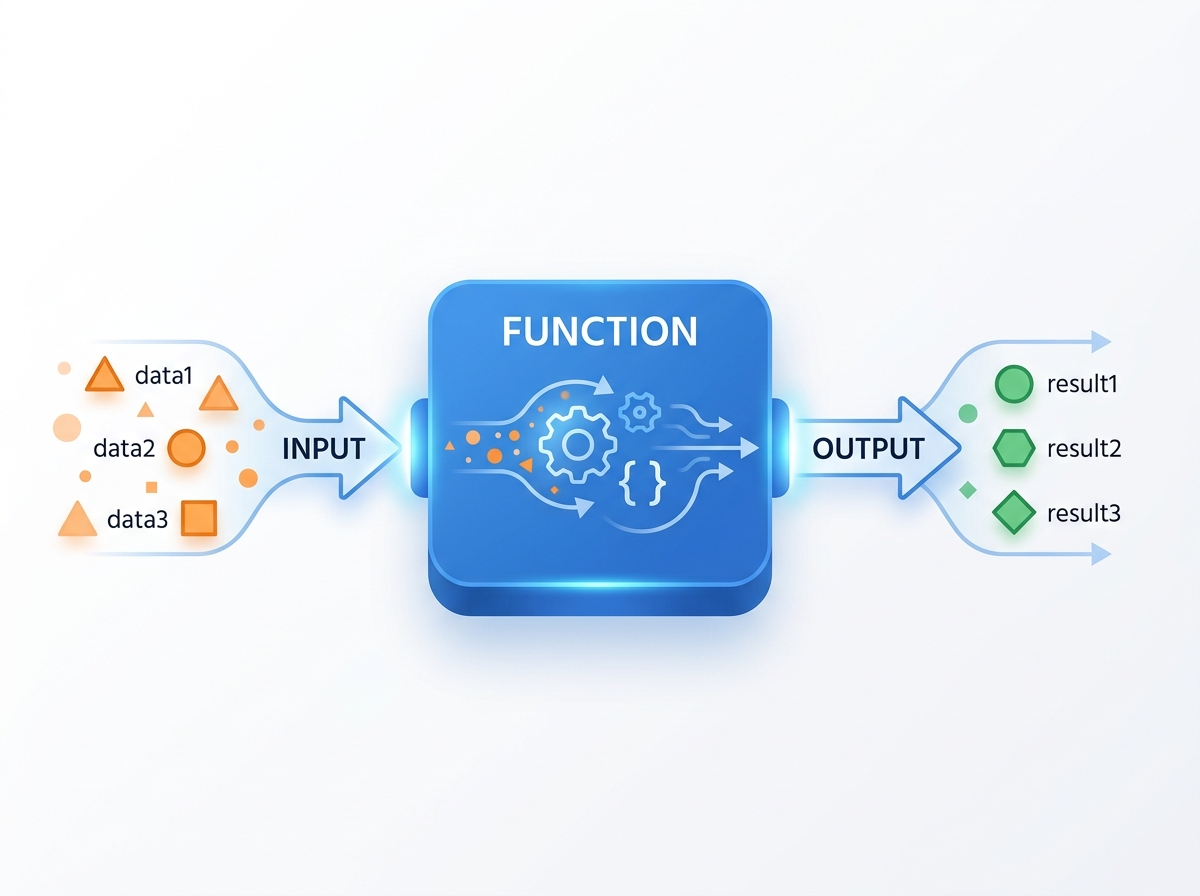
\includegraphics[width=0.8\textwidth]{diagrama_funcao.jpg} \\
                \footnotesize{Entrada (IP/Dados) $\rightarrow$ Processamento $\rightarrow$ Saída (Resultado)}
            \end{center}
        \end{column}
    \end{columns}
\end{frame}

\begin{frame}[fragile]{Como Definir uma Função em Python}
    Para criar uma função, usamos a palavra-chave \textbf{def} (de \textit{define} ou definir), seguida pelo nome da função, parênteses e dois pontos.
    
    \begin{lstlisting}[language=Python]
def nome_da_funcao(parametro1, parametro2):
    # Corpo da funcao (o que ela faz)
    # Codigo identado
    return resultado # Opcional
    \end{lstlisting}
    
    \vspace{0.3cm}
    \textbf{Regras importantes:}
    \begin{itemize}
        \item O nome deve ser explicativo (ex: \texttt{verificar\_conexao}).
        \item O bloco de código interno \textbf{deve estar identado} (com 4 espaços).
        \item Para executar a função, nós a ``chamamos'' pelo nome: \texttt{nome\_da\_funcao()}.
    \end{itemize}
\end{frame}
